Web Services bieten eine auf Standards basierende Technologie, um SOAs zu realisieren. Mittlerweile setzen viele gro�e Softwarekonzerne auf Web Services und haben ihre Produktstrategien entsprechend ausgerichtet.

Als Web-Service bezeichnet man im Allgemeinen eine Softwarekomponente, die
ihre Funktionalit�at �uber Standardinternetprotokolle zur Verf�ugung stellt.
W3C definiert die Web Services folgenderma�en: 
\begin{Def}
A software application identified by a URI, whose interfaces and bindings are capable of being
defined, described, and discovered as XML artifacts. A Web service supports direct interactions
with other software agents using XML-based messages exchanged via Internet-based protocols.(W3C)
\end{Def}

a.) Ein Web Service wird durch einen URI identifiziert.1
b.) Die Schnittstelle eines Web Services ist maschinenlesbar und wird durch
WSDL (siehe n�chsten Abschnitt) beschrieben.
c.) Ein Web Service kommuniziert mit anderen Softwarekomponenten durch
XML Nachrichten. Der Nachrichtenaustausch kann insbesondere mit Hilfe
von Internetprotokollen (z.B. HTTP oder SMTP) stattfinden.

W�hrend die erste Definition die konkreten Interaktionsprotokollen und Beschreibungssprache f�r die Schnittstellen noch offen l�sst, werden in der n�chste Definition die  geeigneten Standards genannt. 
\begin{Def}
A Web service is a software system designed to support interoperable machine-to-machine
interaction over a network. It has an interface described in a machine-processable format
(specifically WSDL). Other systems interact with the Web service in a manner prescribed by its
description using SOAP messages, typically conveyed using HTTP with an XML serialization in
conjunction with other Web-related standards (W3C 2004a).
\end{Def}

Gem�� der beiden Definitionen sind die Beschreibung von Schnittstellen und
der Nachrichtenaustausch wesentliche Aufgaben. SOAP, WSDL und UDDI sind die daf�r vorgesehen Standards und bilden den Kern der Web Services.
\begin{itemize}
	\item SOAP ein standardisiertes, XML-basiertes
Protokoll zum Verpacken von Nachrichten, die zwischen Applikationen ausgetauscht
werden. SOAP setzt auf Transportschicht auf und ist von dem verwendetetn Transportprotokoll unabh�ngig. Am H�ufigsten wird der HTTP-Protokoll eingesetzt.
\item UDDI (Universal Description, Discovery and Integration) dient zur Lokalisierung und Ver�ffentlichung
von Web-Services im Internet. UDDI bietet Standardfunktionen zum Klassifizieren,
Katalogisieren und Verwalten von Metadaten �ber Web-
Services.
\item WSDL (Web Services Defnition Language) ist eine funktionale, XML-basierte Beschreibungssprache
f�r die Schnittstellen eines Web Services.(siehe n�chsten Abschnitt)
\end{itemize}

Der Zusammenhang dieser Standards und die grundlegende Funktionsweise ist in der Abbildung \ref{fig:WSFunktionsweise} dargestellt.
\begin{figure}[htbp]
	\centering
		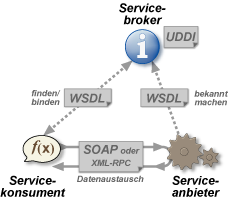
\includegraphics[width=0.6\textwidth]{bilder/Webservice.png}
		\caption{Kontrollfluss eines BPEL Prozesses}
	\label{fig:WSFunktionsweise}
\end{figure}


Weier M�glichkeit..........

Die Abbildung \ref{fig:wsTechnologieStack} zeigt den Web Service Technologie Stack.  

\begin{figure}[htbp]
	\centering
		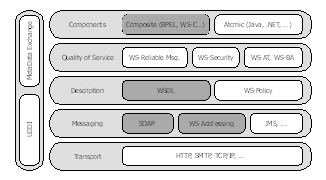
\includegraphics[width=0.7\textwidth]{bilder/wsTechnologieStack.png}
		\caption{Web Service Technologie Stack}
	\label{fig:wsTechnologieStack}
\end{figure}